\documentclass[a4paper,12pt,oneside]{book}

%-------------------------------Start of the Preable------------------------------------------------
\usepackage[english]{babel}
\usepackage{tocloft}

\renewcommand\cftchapafterpnum{\vskip10pt}
\renewcommand\cftsecafterpnum{\vskip15pt}
\usepackage{blindtext}
%packagr for hyperlinks
\usepackage{hyperref}
\hypersetup{
    colorlinks=true,
    linkcolor=black,
    filecolor=magenta,      
    urlcolor=cyan,
}

\urlstyle{same}
%use of package fancy header
\usepackage{fancyhdr}
\setlength\headheight{26pt}
\fancyhf{}
%\rhead{
\includegraphics[width=1cm]{logo}}
\lhead{\rightmark}
\rhead{
\includegraphics[width=1cm]{logo}}
\fancyfoot[RE, RO]{\thepage}
\fancyfoot[CE, CO]{\href{http://www.e-yantra.org}{www.e-yantra.org}}

\pagestyle{fancy}

%use of package for section title formatting
\usepackage{titlesec}
\titleformat{\chapter}
  {\Large\bfseries} % format
  {}                % label
  {0pt}             % sep
  {\huge}           % before-code
 
%use of package tcolorbox for colorful textbox
\usepackage[most]{tcolorbox}
\tcbset{colback=cyan!5!white,colframe=cyan!75!black,halign title = flush center}

\newtcolorbox{mybox}[1]{colback=cyan!5!white,
colframe=cyan!75!black,fonttitle=\bfseries,
title=\textbf{\Large{#1}}}

%use of package marginnote for notes in margin
\usepackage{marginnote}

%use of packgage watermark for pages
%\usepackage{draftwatermark}
%\SetWatermarkText{
\includegraphics{logo}}
\usepackage[scale=2,opacity=0.1,angle=0]{background}
\backgroundsetup{
contents={
\includegraphics{logo}}
}

%use of newcommand for keywords color
\usepackage{xcolor}
\newcommand{\keyword}[1]{\textcolor{red}{\textbf{#1}}}

%package for inserting pictures
\usepackage{graphicx}

%package for highlighting
\usepackage{color,soul}

%new command for table
\newcommand{\head}[1]{\textnormal{\textbf{#1}}}


%----------------------End of the Preamble---------------------------------------


\begin{document}

%---------------------Title Page------------------------------------------------
\begin{titlepage}
\raggedright
{\Large eYSIP2016\\[1cm]}
{\Huge\scshape WEB MONITORING FOR GREENHOUSE \\[.1in]}

\vfill

        {\underline{\large{Interns:}}} \\
        \begin{quote}
        	\large{Ankit Gala}
        	
        	\large{Email: ankitg444@gmail.com}		
        	
        	\large{Mobile: 7208760344}
        \end{quote}
        
        
		
		\begin{quote}
			\large{Neel Rami}
        	
        	\large{Email: neelrami911@gmail.com}	
        	
        	\large{Mobile: 9029585939}
		\end{quote}
        
        
        \vspace{0.5cm}
        
          {\underline{\textbf{Mentors:}}} \\
          \begin{quote}
          \large{Jayant Solanki}
          
          \large{Email: jayantjnp@gmail.com}
          \end{quote}
          
          

\begin{flushright}
{\large Duration of Internship: $ 21/05/2016-10/07/2016 $ \\}

\end{flushright}
{\itshape 2016, e-Yantra Publication}



\end{titlepage}

\tableofcontents
%-------------------------------------------------------------------------------
\chapter[Web Monitoring For Greenhouse]{Web Monitoring For Greenhouse}
\section{Abstract}
\hspace{7mm}This project aims at developing a web portal with the help of which various aspects of the greenhouse such as scheduling a task,switching irrigation valves,visualizing data collected from various devices,managing devices and displaying their status can be controlled and monitored by any user.\\

With the help of this web portal,anyone can remotely access various aspects of greenhouse and control it.This project aims at providing automation to greenhouse systems.\\

The ultimate goal of the project would be to eliminate the user from manually controlling various aspects of greenhouse and provide effective automation through the Internet-of-things approach.

\newpage

\section{Completion status}
\begin{itemize}
    \item{Task Accomplished}
    \setlength\itemsep{0.2cm}
        \begin{enumerate}
            \item{Understanding the current back-end system of the Greenhouse.}
            \item{Study of Bower,AngularJS,Websocket}
            \item{Installation of required software.}
            \item{Creating Login and Signup pages.}
            \item{Creating an Admin page for managing users.}
            \item{Creating Device Management page.}
            \item{Designing a Device Status page with dynamic update.}
            \item{Controlling irrigation valves using Websocket.}
            \item{Understanding JavaScript based Charts APIs.}
            \item{Plotting charts for multiple data.}
            \item{ Designing a Scheduling Page.}
            \item{Understanding RTSP.}
            \item{Designing dashboard}
            \item{Code Documentation and Project Report.}
        \end{enumerate}
    \item{Task Uncompleted}
        \begin{enumerate}
            \item{Designing page for Live Video Feed.}
        \end{enumerate}
        \par In order to embed RTSP live video feed in webpage,plugins should be used.But the major problem with plugins is that they are browser and OS dependent.Also there is no specific Javascript library which can be used to embed live videos in webpage.So its difficult to embed RTSP live video feed in a webpage.   
\end{itemize}


\newpage
\section{Hardware parts}
\hspace{7mm}No Hardware parts used.

\section{Software used}
\begin{enumerate}
    \item Linux Environment
        \begin{itemize}
            \item Setting up the System 
                \begin{enumerate}
                    \item Software used:Ubuntu OS
                    \item Version:Ubuntu 15.04
                    \item \href{http://old-releases.ubuntu.com/releases/15.04/}{Ubuntu 15.04 Download Link}
                \end{enumerate}
            \item Setting up the Server
                \begin{enumerate}
                    \item Software used:
                        \begin{itemize}
                            \item Apache
                            \item PHP
                        \end{itemize}
                    \item Version:
                        \begin{itemize}
                            \item{Apache version-2.4.10}
                            \item{PHP version-5.6.4}
                        \end{itemize}
                    \item Installation Commands:
                        \begin{itemize}
                            \item{Apache: \\
                            sudo apt-get update\\
                            sudo apt-get install apache2}
                            \item {PHP:\\
                            sudo apt-get install php5 libapache2-mod-php5 php5-mcrypt}
                        \end{itemize}
                \end{enumerate}
            \item Setting up the Database
                \begin{enumerate}
                    \item Software used:MYSQL
                    \item Installation command: \\sudo apt-get install mysql-server libapache2-mod-auth-mysql php5-mysql
                \end{enumerate}
            \item{Setting up package manager}
                \begin{enumerate}
                    \item{Software used:Bower}
                    \item{Note:Bower requires node, npm and git.}
                    \item {Installation command: npm install -g bower}
                \end{enumerate}
            \item{Setting up essential libraries}
                \begin{enumerate}
                    \item{Jquery}
                        \begin{itemize}
                            \item{Installation command: bower install jquery}
                        \end{itemize}
                    \item{Bootstrap}
                        \begin{itemize}
                            \item{Installation command: bower install bootstrap}
                        \end{itemize}
                    \item{AngularJS}
                        \begin{itemize}
                            \item{Installation command: bower install angular}
                        \end{itemize}
                    \item{Angular Material}
                        \begin{itemize}
                            \item{Installation command: bower install angular-material}
                        \end{itemize}
                    \item{amCharts}
                        \begin{itemize}
                            \item{Installation command: bower install amcharts3}
                        \end{itemize}
                    \item{angular-animate}
                        \begin{itemize}
                            \item{Installation command: bower install angular-animate}
                        \end{itemize}
                    \item{angular-aria}
                        \begin{itemize}
                            \item{Installation command: bower install angular-aria}
                        \end{itemize}
                    \item{angular-ui}
                        \begin{itemize}
                            \item{Installation command: bower install angular-bootstrap}
                        \end{itemize}
                    \item{angular-datatables}
                        \begin{itemize}
                            \item{Installation command: bower install angular-datatables}
                        \end{itemize}
                    \item{angular-pagination}
                        \begin{itemize}
                            \item{Installation command: bower install angular-utils-pagination}
                        \end{itemize}
                \item{bootstrap-table}
                    \begin{itemize}
                        \item{Installation command: bower install bootstrap-table}
                    \end{itemize}
                \item{DataTables}
                    \begin{itemize}
                        \item{Installation command: bower install }
                    \end{itemize}
                \item{mmenu}
                    \begin{itemize}
                        \item{Installation command: bower install jquery-mmenu}
                    \end{itemize}
            \end{enumerate}
    \end{itemize}
    \item Windows Environment
    \begin{itemize}
        \item Setting up the environment
            \begin{enumerate}
            \item Software used:Windows OS
            \item Version:Windows 7 Premium
            \item \href{https://www.microsoft.com/en-in/software-download/windows7}{Windows 7 Download Link}
        \end{enumerate}
        \item Setting up the Server \& Database
            \begin{enumerate}
                \item Software used:XAMPP
                \item Version:XAMPP version 3.2.2
                \item \href{https://www.apachefriends.org/download.html}{XAMPP Download Link}
            \end{enumerate}
        \item Setting up the Editor
            \begin{enumerate}
                \item Software used:Sublime Text
                \item \href{https://www.sublimetext.com/}{Sublime Text Download Link}
            \end{enumerate}
        \item{Setting up package manager}
            \begin{enumerate}
                \item{Software used:Bower}
                \item{Note:Bower requires node, npm and git.}
                \item {Installation command: npm install -g bower}
                \item{Note:The above installation command should be wriiten in Git Bash.}
            \end{enumerate}
        \item{Setting up essential libraries}
            \begin{enumerate}
                    \item{Jquery}
                        \begin{itemize}
                            \item{Installation command: bower install jquery}
                        \end{itemize}
                    \item{Bootstrap}
                        \begin{itemize}
                            \item{Installation command: bower install bootstrap}
                        \end{itemize}
                    \item{AngularJS}
                        \begin{itemize}
                            \item{Installation command: bower install angular}
                        \end{itemize}
                    \item{Angular Material}
                        \begin{itemize}
                            \item{Installation command: bower install angular-material}
                        \end{itemize}
                    \item{amCharts}
                        \begin{itemize}
                            \item{Installation command: bower install amcharts3}
                        \end{itemize}
                    \item{angular-animate}
                        \begin{itemize}
                            \item{Installation command: bower install angular-animate}
                        \end{itemize}
                    \item{angular-aria}
                        \begin{itemize}
                            \item{Installation command: bower install angular-aria}
                        \end{itemize}
                    \item{angular-ui}
                        \begin{itemize}
                            \item{Installation command: bower install angular-bootstrap}
                        \end{itemize}
                    \item{angular-datatables}
                        \begin{itemize}
                            \item{Installation command: bower install angular-datatables}
                        \end{itemize}
                    \item{angular-pagination}
                        \begin{itemize}
                            \item{Installation command: bower install angular-utils-pagination}
                        \end{itemize}
                \item{bootstrap-table}
                    \begin{itemize}
                        \item{Installation command: bower install bootstrap-table}
                    \end{itemize}
                \item{DataTables}
                    \begin{itemize}
                        \item{Installation command: bower install }
                    \end{itemize}
                \item{mmenu}
                    \begin{itemize}
                        \item{Installation command: bower install jquery-mmenu}
                    \end{itemize}
            \end{enumerate}
    \end{itemize}
  

\section{Assembly of hardware}
\hspace{7mm}No Hardware parts used



\section{Software and Code}
\hspace{7mm}\href{https://github.com/eYSIP-2016/eYSIP-2016-Web-Monitoring-For-Greenhouse}{Github link} for the repository of code.\\

{\underline{Code Explanation}}:\\
\begin{itemize}
    \setlength\itemsep{0.2cm}
    \item{Current Greenhouse Setup:}
        \begin{itemize}
            \item{Current Greenhouse has columns of troughs containing plants.}
            \item{Current hardware setup at the Greenhouse has two types of devices, one controls the irrigation valves and the other gets the temperature, humidity, moisture values.}
            \item{The first type controls 1-10 Irrigation valves at a time.}
            \item{The second type of device also known as Sensor nodes gathers the environment values.}
            \item{Irrigation valves and the sensor nodes are placed at every troughs and are placed in different groups.}
        \end{itemize}
        
        
    \item{Database Structure Explanation: }
    \begin{itemize}
        \item{devices table: Stores information related to a device such as name,deviceid,description,type etc. }
        \item{devicestatus table :Stores connectivity status of a device.}
        \item{feeds table: Stores data such as battery,temperature,moisture etc of a device.}
        \item{groups table: Stores various groups.}
        \item{security\_questions table: Stores security question and corresponding id.}
        \item{switches table: Stores status of a valve's switch.}
        \item{sensors table: Stores device types.}
        \item{tasks table: Stores various schedules created by user or machine.}
        \item{users table: Stores user login credentials.}
    \end{itemize}
    \newpage
    \item{Features:}
        \begin{enumerate}
        \setlength\itemsep{0.2cm}
            \item{Registration and Authentication}
                \begin{itemize}
                \setlength\itemsep{0.2cm}
                    
                    \item{Website supports two types of users.}
                        \begin{enumerate}
                            \item{Administrative User}
                            \item{Normal User}
                        \end{enumerate}
                    \item{A user won't be able to access any page unless his/her account has been activated by any administrative user.}
                    \item{If his/her account has been activated by the admin,he/she will be directed to the dashboard.}
                    \item{Efforts have been made to implement a strong password policy.}
                    \item{Password Reset procedure has been implemented using a security question.}
                    \item{During the registration procedure,the user has to select a security question and answer that question.}
                    \item{If a user forgets the password,then he/she has to answer the security question.}
                    \item{If a user forgets his/her username or email or security question's answer,then he/she has to create a new account.}
                    \item{The essential credentials such as password and security question's answer are encrypted an then stored in database.}
                    \item{Accessible to both normal as well as administrative users.}
                        
                \end{itemize}
                \vspace{0.3cm}
            \item{Managing Users}
            \begin{itemize}
            \setlength\itemsep{0.2cm}
                \item{Accessible only to administrative users.}
                \item{Four types of accounts.}
                    \begin{enumerate}
                        \item{Normal User Account}
                        \item{Administrative User Account}
                        \item{Pending Approval Account }
                        \item{De-activated Account}
                    \end{enumerate}
                \item{Once a user creates an account,his account will be in pending approval state.}
                \item{If his/her account is activated by any administrative user,then he/she would be able to access the web portal.}
                \item{Any administrative user can promote a normal user and make him an administrative user.}
                \item{Any administrative user can demote another administrative user into a normal user.}
                \item{Any administrative user can de-activate another administrative user's account or normal user's account.}
            \end{itemize}
            \vspace{0.3cm}
            \item{Device Management}
                \begin{itemize}
                    \item{Accessible to both normal as well as administrative users.}
                    \item{This page helps to manage various devices.}
                    \item{This page displays basic information of a device such as its name,type,latitude,longitude etc.}
                    \item{We can even edit information of any device such as editing its name,group,device type etc..}
                    \item{The page provides facility for adding a new group and also editing an existing group.}
                     \item{It also provides facility for adding a device type and also editing an existing device type.}
                \end{itemize}
             \item{Device Status}
                \begin{itemize}
                \item{Accessible to both normal as well as administrative users.}
               \item{The purpose of this page is for monitoring various devices.}
               \item{Various types of data such as primary battery and secondary battery for valves and battery value and moisture value for sensor nodes are being displayed on this page.}
              \item{Also connectivity status i.e whether the device is online or offline is being indicated on this page.}
               \item{The page also shows the time when the device went online or offline.}
               \item{For each valve,the respective switches and their status i.e whether the switch is open or close has also been demonstrated on the page.}
               \item{First the user has to select a particular group and the devices belonging to those groups and their respective data is displayed on the page.}
                \item{All the data such as battery value,connectivity status,switch status etc. is dynamically updated using Websockets.}
           \end{itemize}
            
            \item{Controlling Valves}
            \setlength\itemsep{0.2cm}
                \begin{itemize}
                    \item{Accessible to both normal as well as administrative users.}
                    \item{The page aims at controlling irrigation valves using the Websocket.}
                    \item{Any user can easily switch on or switch off an individual switch of any valve.}
                    \item{The user can also specify the duration for which a particular switch of a valve should be switched on.}
                    \item{First,the user has to select appropriate group.}
                    \item{If he wants to open a switch,he can also specify the duration and then simply open the switch.}
                \end{itemize}
                
            \item{Scheduling Page}
            \setlength\itemsep{0.2cm}
                \begin{itemize}
                    \item{Accessible to both normal as well as administrative users.}
                    \item{This page displays all the scheduled tasks for a particular group.}
                    \item{The user can also add a schedule for any group with the help of this page.}
                    \item{There are 3 types of schedules:}
                    \setlength\itemsep{0.2cm}
                        \begin{enumerate}
                            \item{Period}
                            \item{Duration}
                            \item{Frequency}
                        \end{enumerate}
                    \item{Steps for adding a schedule: }
                    \setlength\itemsep{0.2cm}
                        \begin{enumerate}
                            \item{Select appropriate group}
                            \item{Select type of schedule}
                            \item{If the selected type of schedule is period, then add start time and end time.}
                            \item{If the selected type is duration,then add start time and the duration of the schedule.}
                            \item{And if the scheduled task is frequency,then add start time,duration and the frequency.}
                        \end{enumerate}
                    \item{Even a schedule can be deleted or disabled.}
                    \item{Later the disabled schedule can be enabled again.}
                    
                    
                \end{itemize}
            \item{Data Visualization}
            \begin{itemize}
                \item{Accessible to both normal as well as administrative users.}
                \item{This page helps the user to visualize several types of data such as battery,moisture,temperature etc in the form of line charts.}
                \item{ Data can also be plotted in real time using websockets and analysed.}
                \item{amCharts,an advanced javascript charting library is used to plot charts.}
                \item{The page has the flexibility to show data on daily,weekly,monthly and yearly basis.}
            \end{itemize}    
           
          
           \item{Dashboard}
            \begin{itemize}
                \item{Accessible to both normal as well as administrative users.}
                \item{This page provides a summarized picture of all the above features.}
            \end{itemize}
            
            \item{Platform Support}
            \begin{itemize}
                
                \item{This web portal supports both desktop as well as mobile version.}
            \end{itemize}
        \end{enumerate}
\end{itemize}

  

\newpage
\section{Use and Demo}
\hspace{7mm}Few glimpses of the Website
\begin{itemize}
\item{Desktop Version}

\vspace{2mm}
Login Page

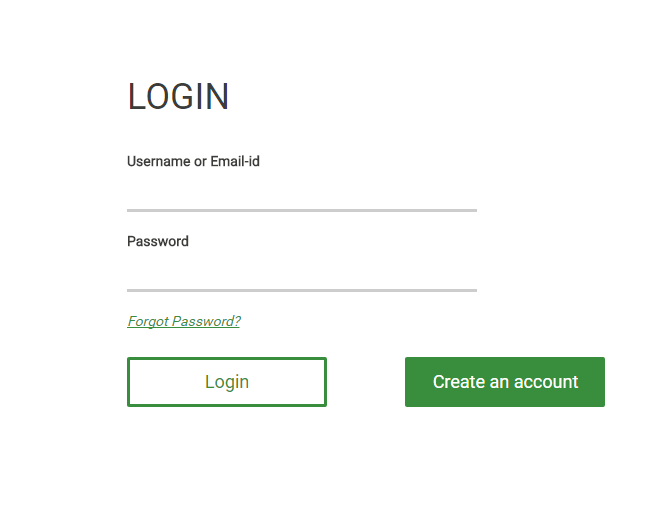
\includegraphics[width=10cm]{logind.png}

\vspace{4mm}
Data Visualization\\


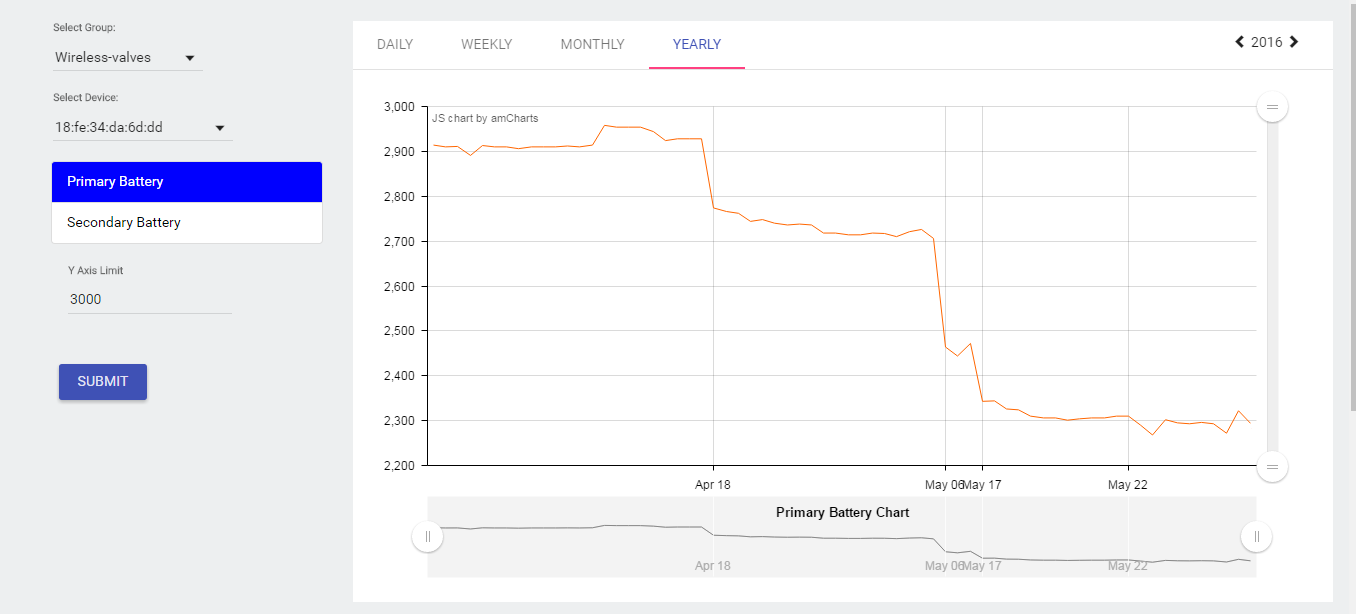
\includegraphics[width=13cm]{chartsd.png}
\newpage
\vspace{3mm}
SignUp Page

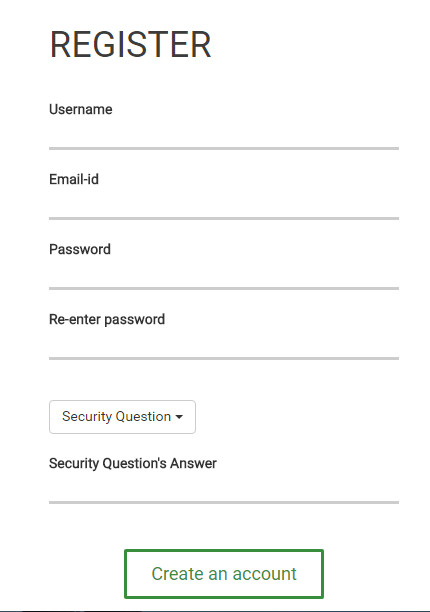
\includegraphics[width=10cm]{signupd.png}
\newpage
\vspace{3mm}
Forgot Password Page

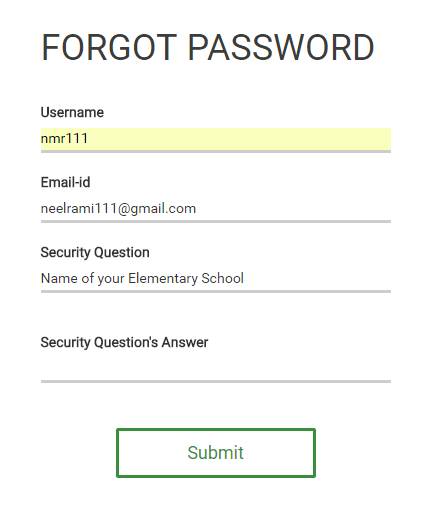
\includegraphics[width=10cm]{fpd.png}

\vspace{3mm}
Device Status Page\\

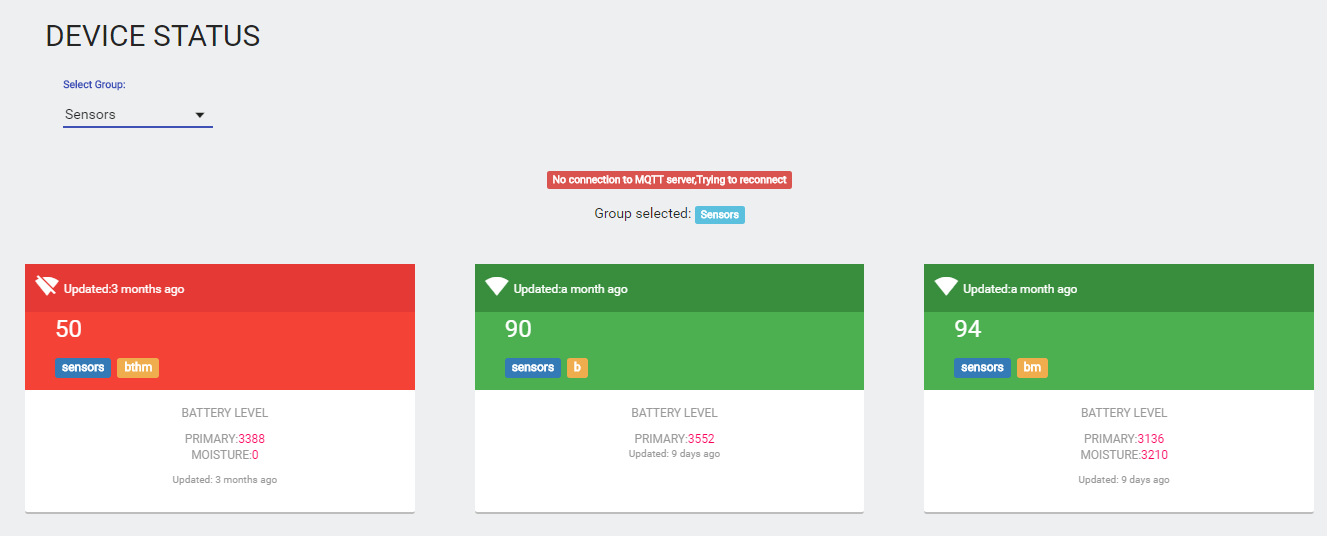
\includegraphics[width=14cm]{devicestatus.png}
\newpage
\vspace{3mm}
Device Management Page\\

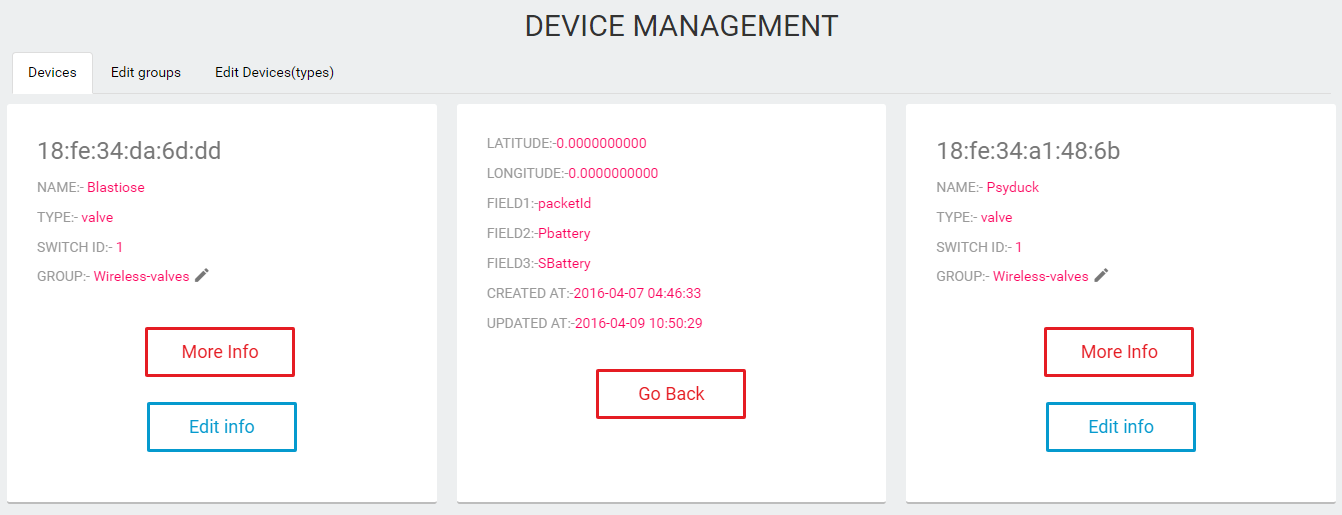
\includegraphics[width=14cm]{devicemanagement1.png}\\




\vspace{3mm}
Valve Control Page\\

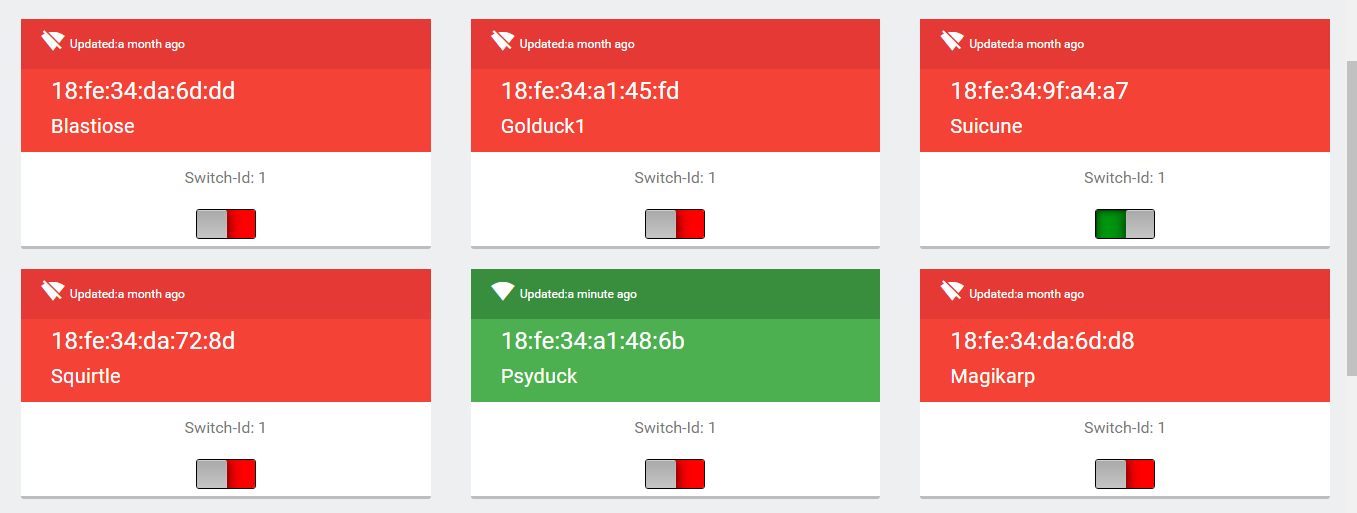
\includegraphics[width=14cm]{valvecontrol1.png}\\

\newpage

\vspace{3mm}
Manage Users Page\\

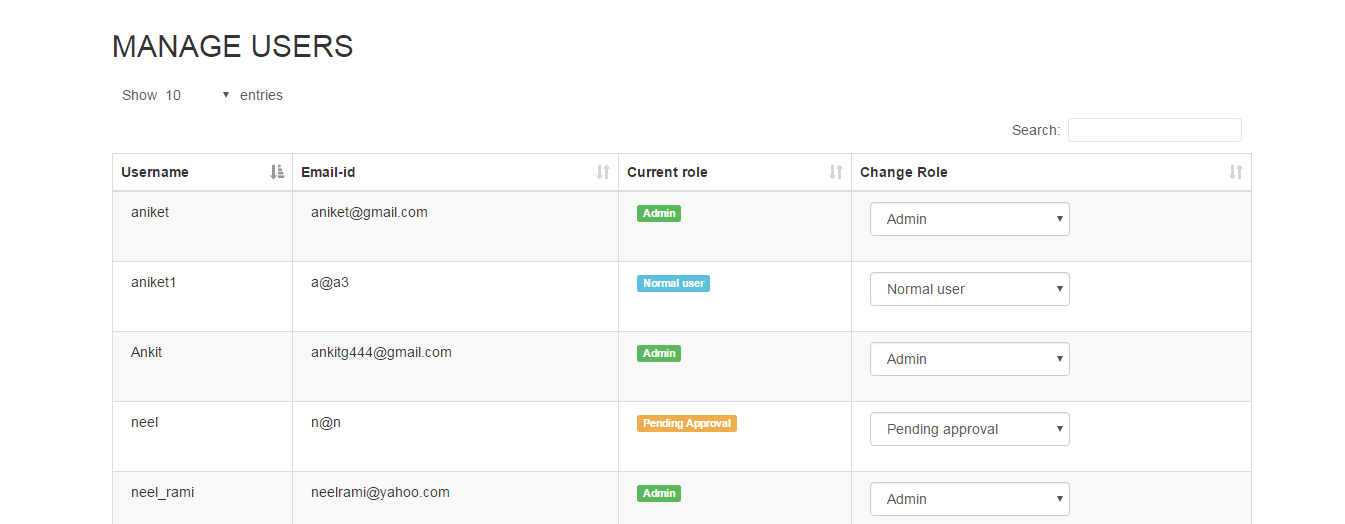
\includegraphics[width=14cm]{manageusersd.png}

\vspace{3mm}
Few Instances Of Dashboard\\

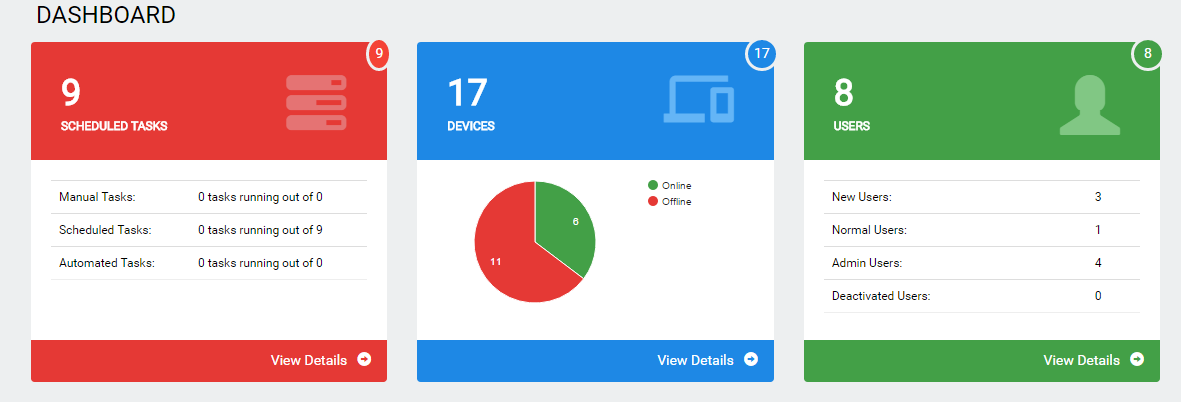
\includegraphics[width=14cm]{dashboard2.png}

\vspace{3mm}
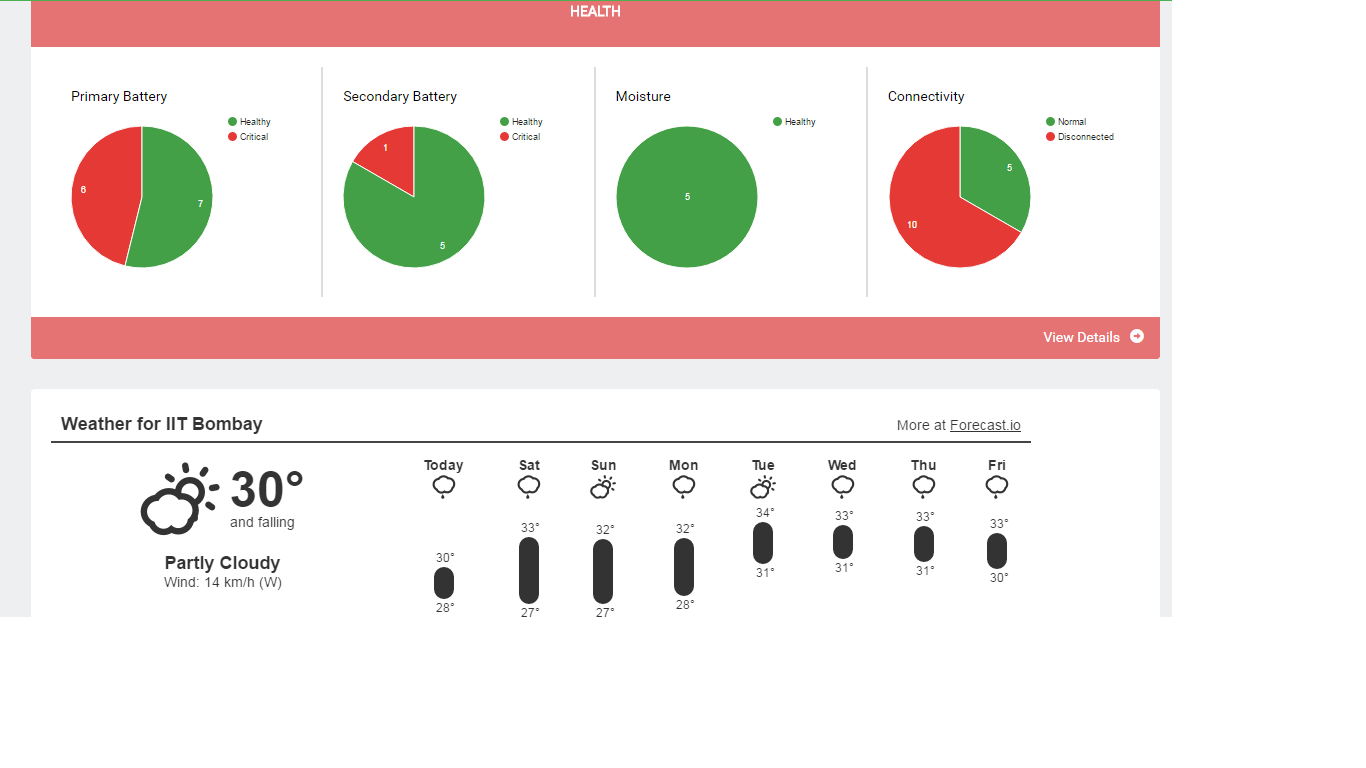
\includegraphics[width=14cm]{dashboard1.png}

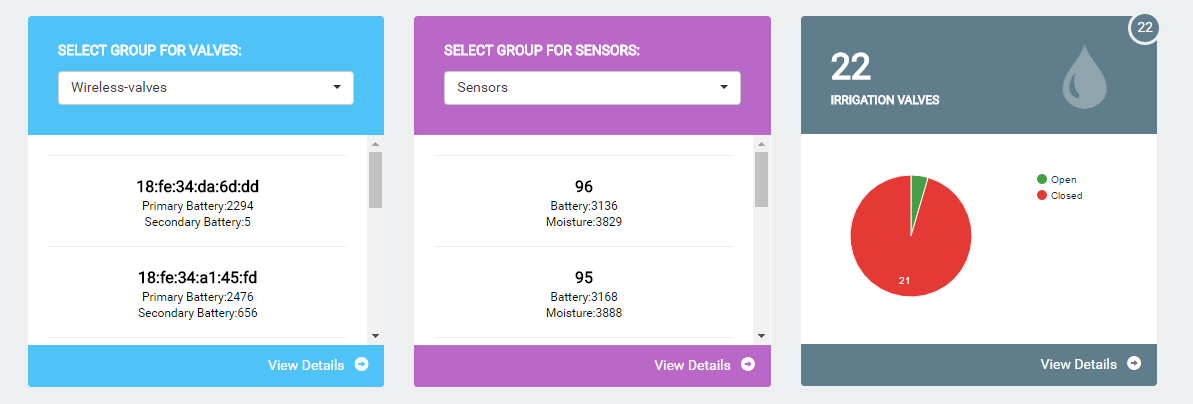
\includegraphics[width=14cm]{dashboard3.png}

\newpage

\item{Mobile Version}\\

Login Page\\

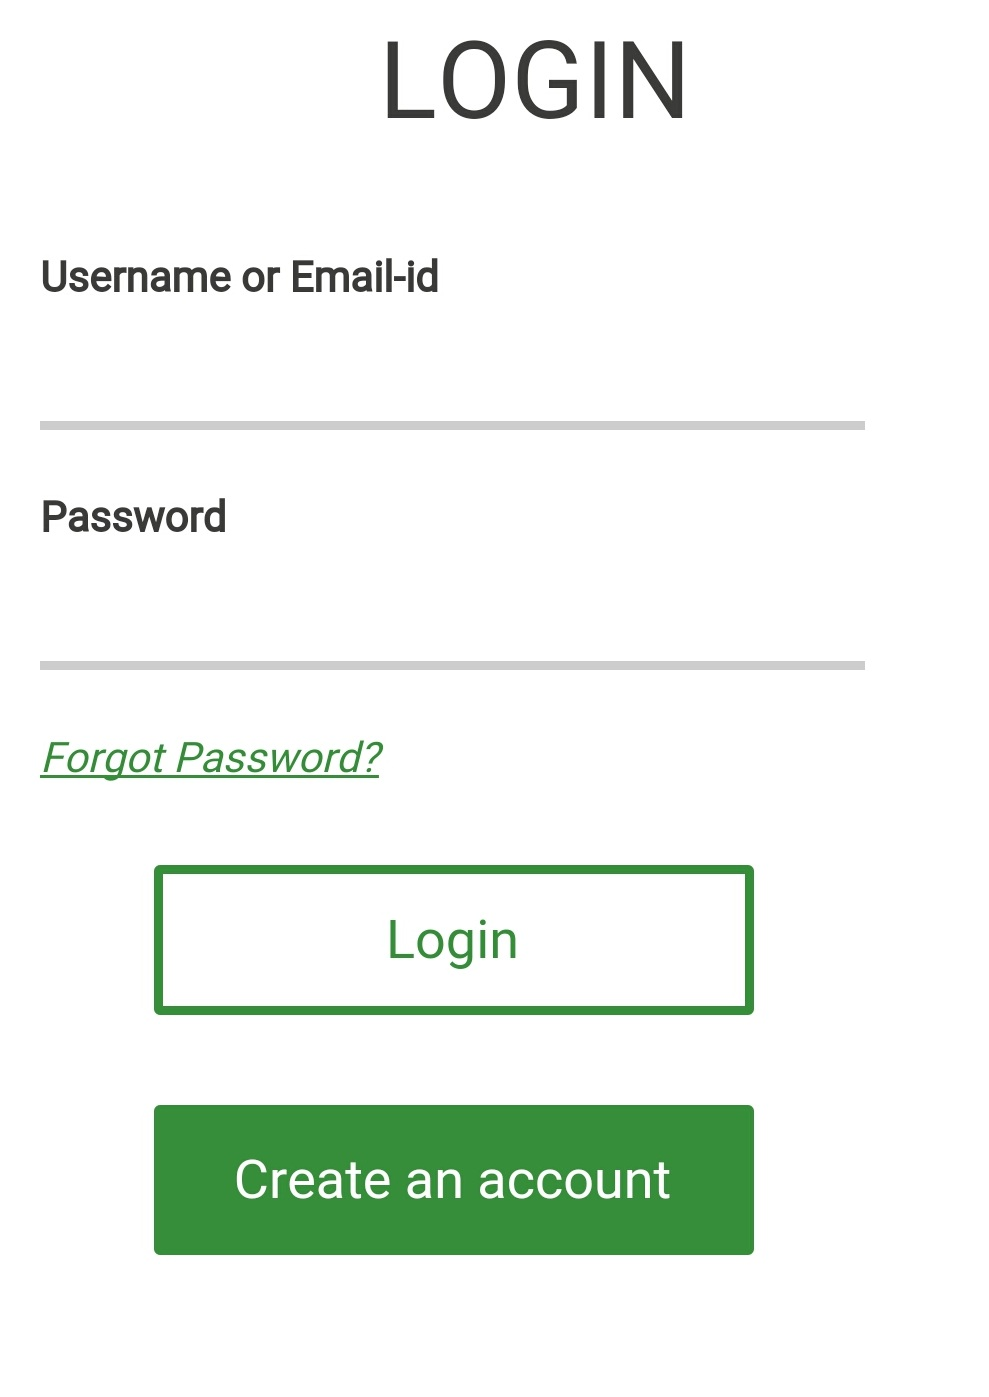
\includegraphics[width=10cm]{loginm.jpg}\\
\newpage
Data Visualization Page\\

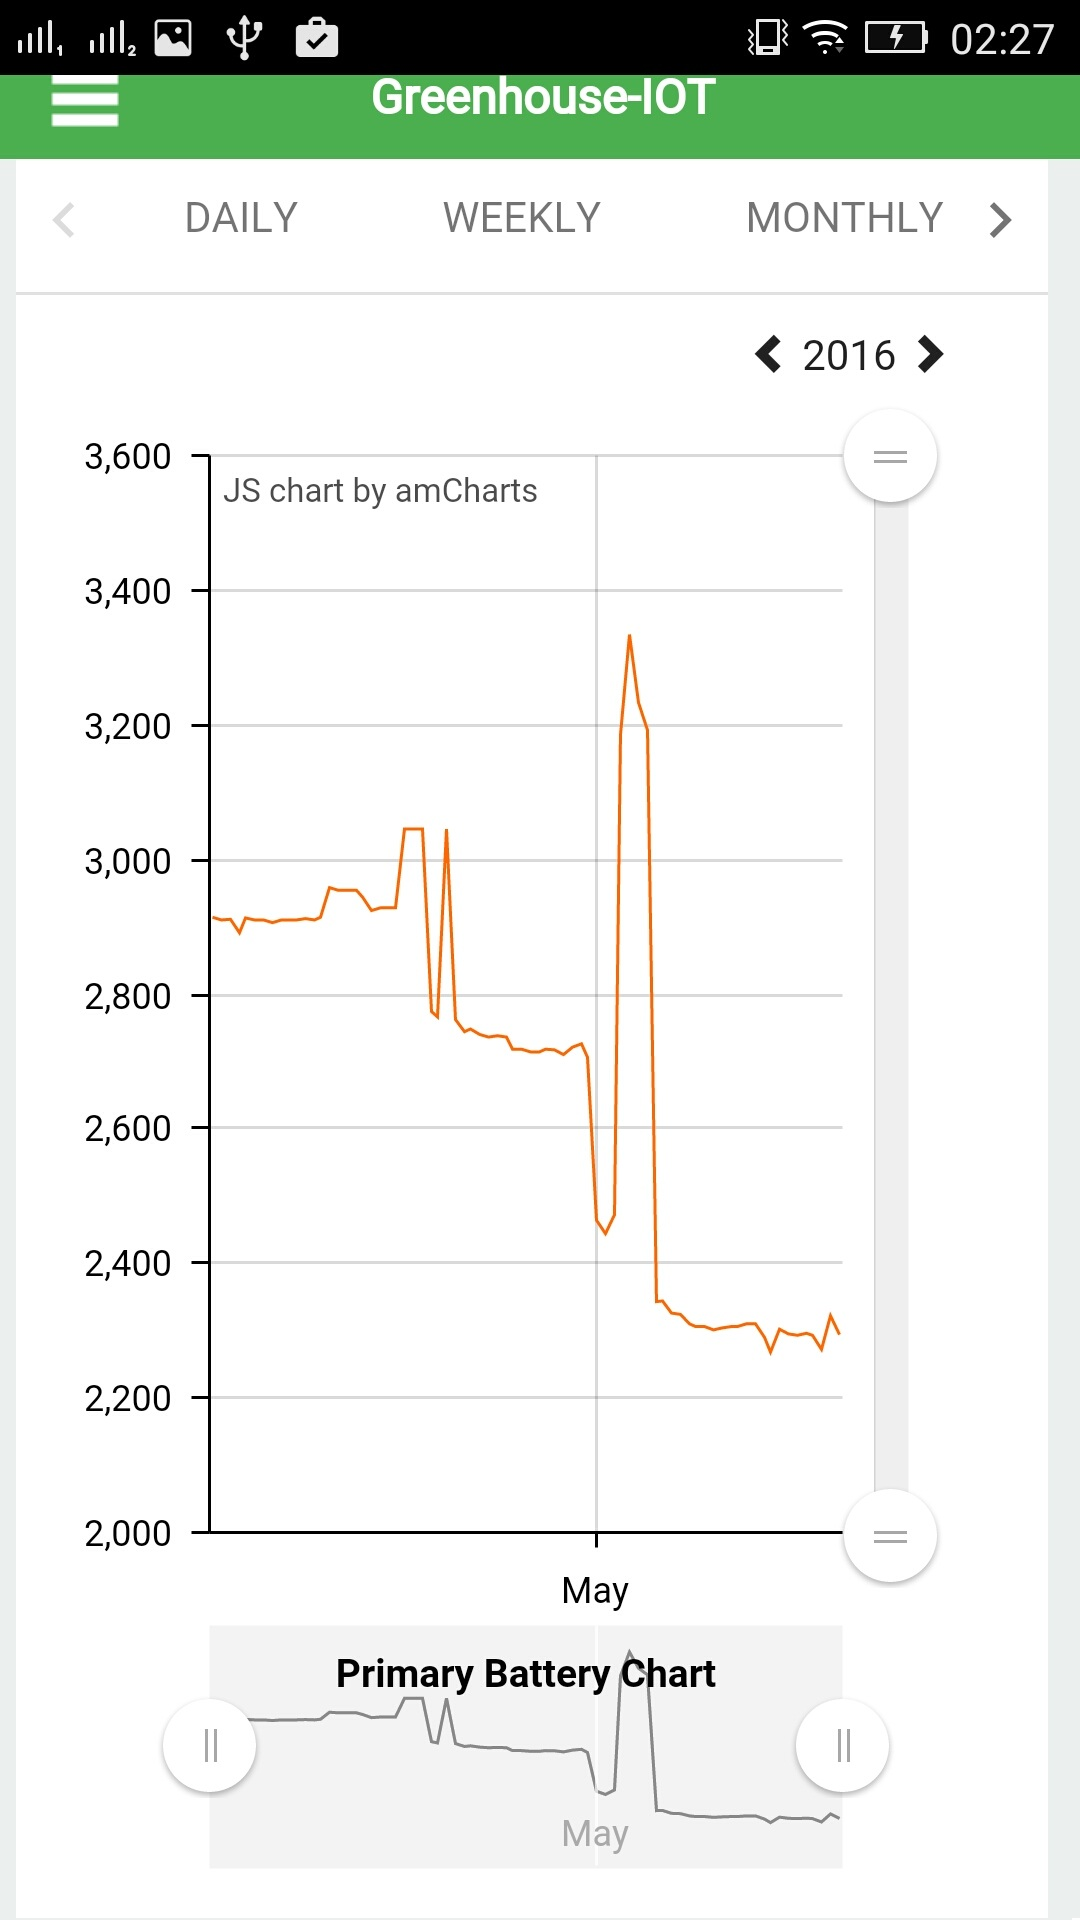
\includegraphics[width=10cm]{chartsm.png}\\
\newpage
Dashboard Page\\

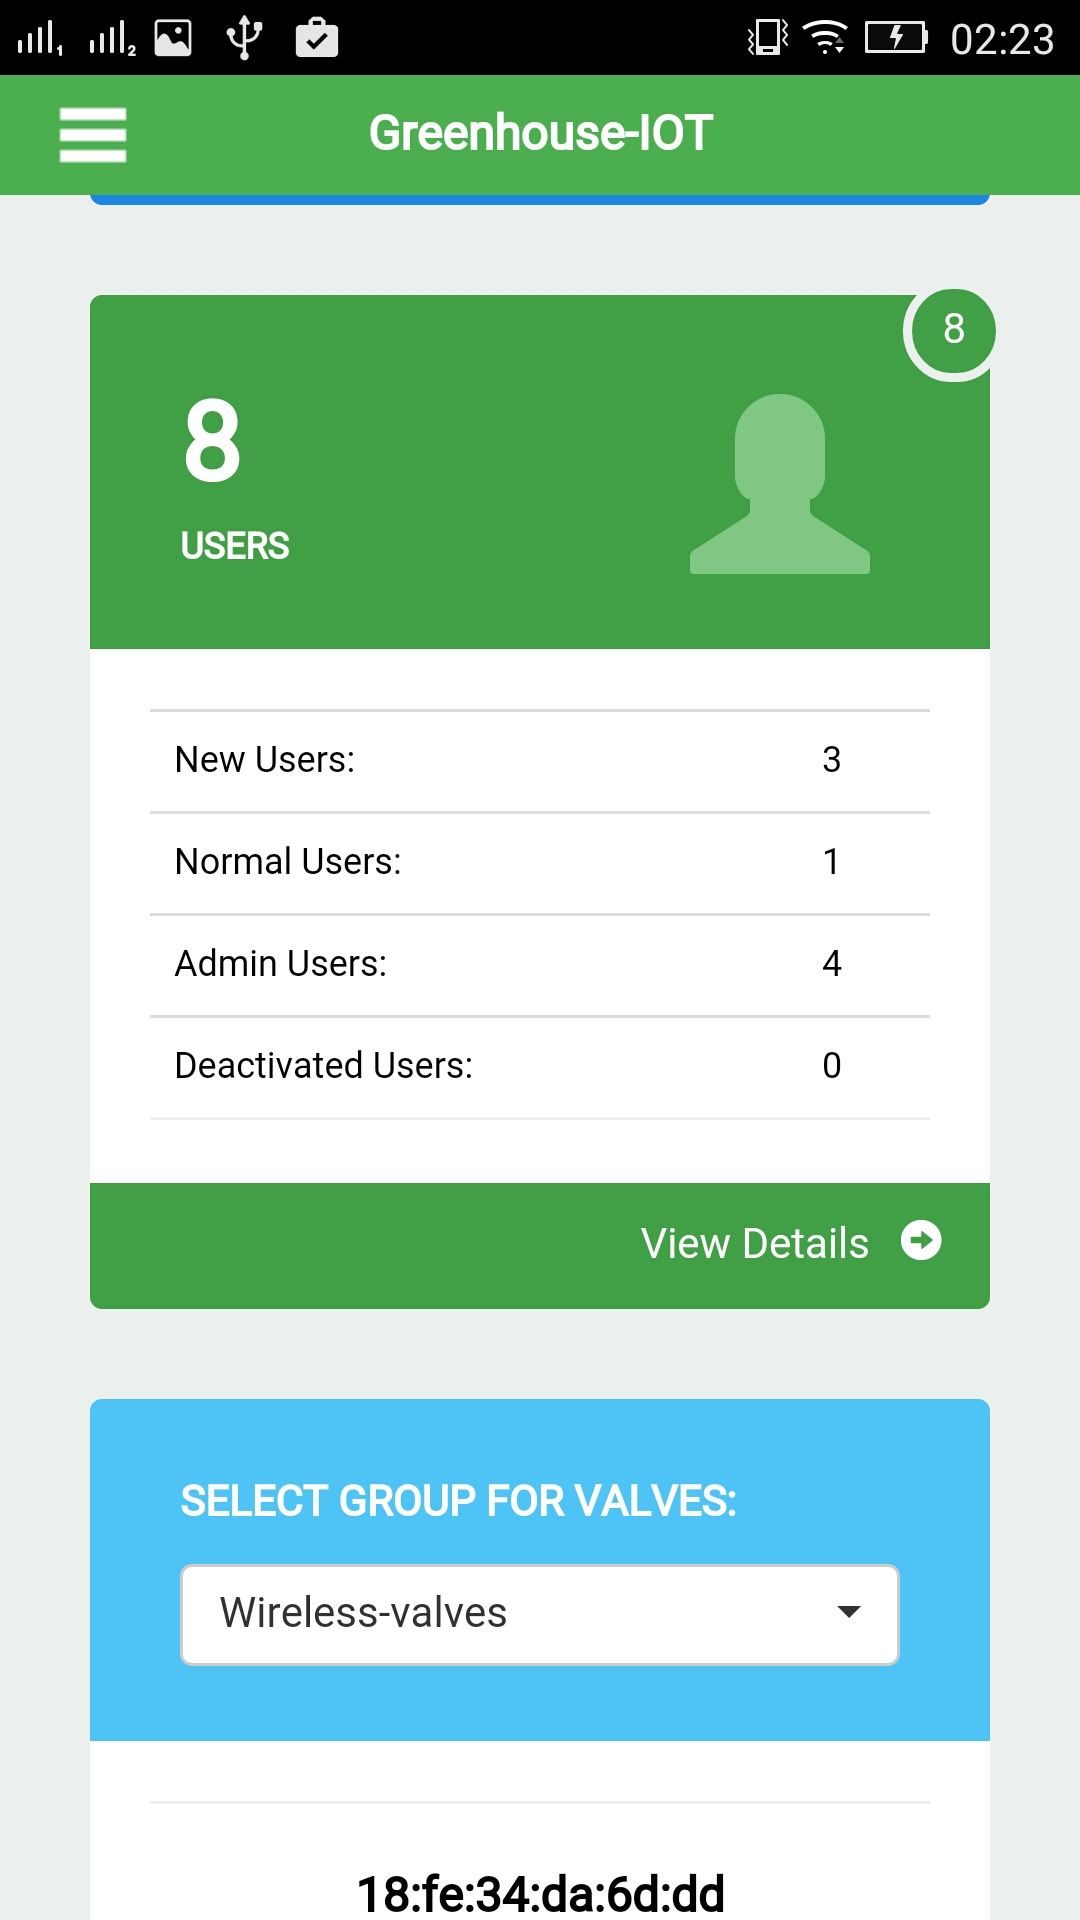
\includegraphics[width=10cm]{dashbaordm2.jpeg}
\newpage
Scheduling Page\\

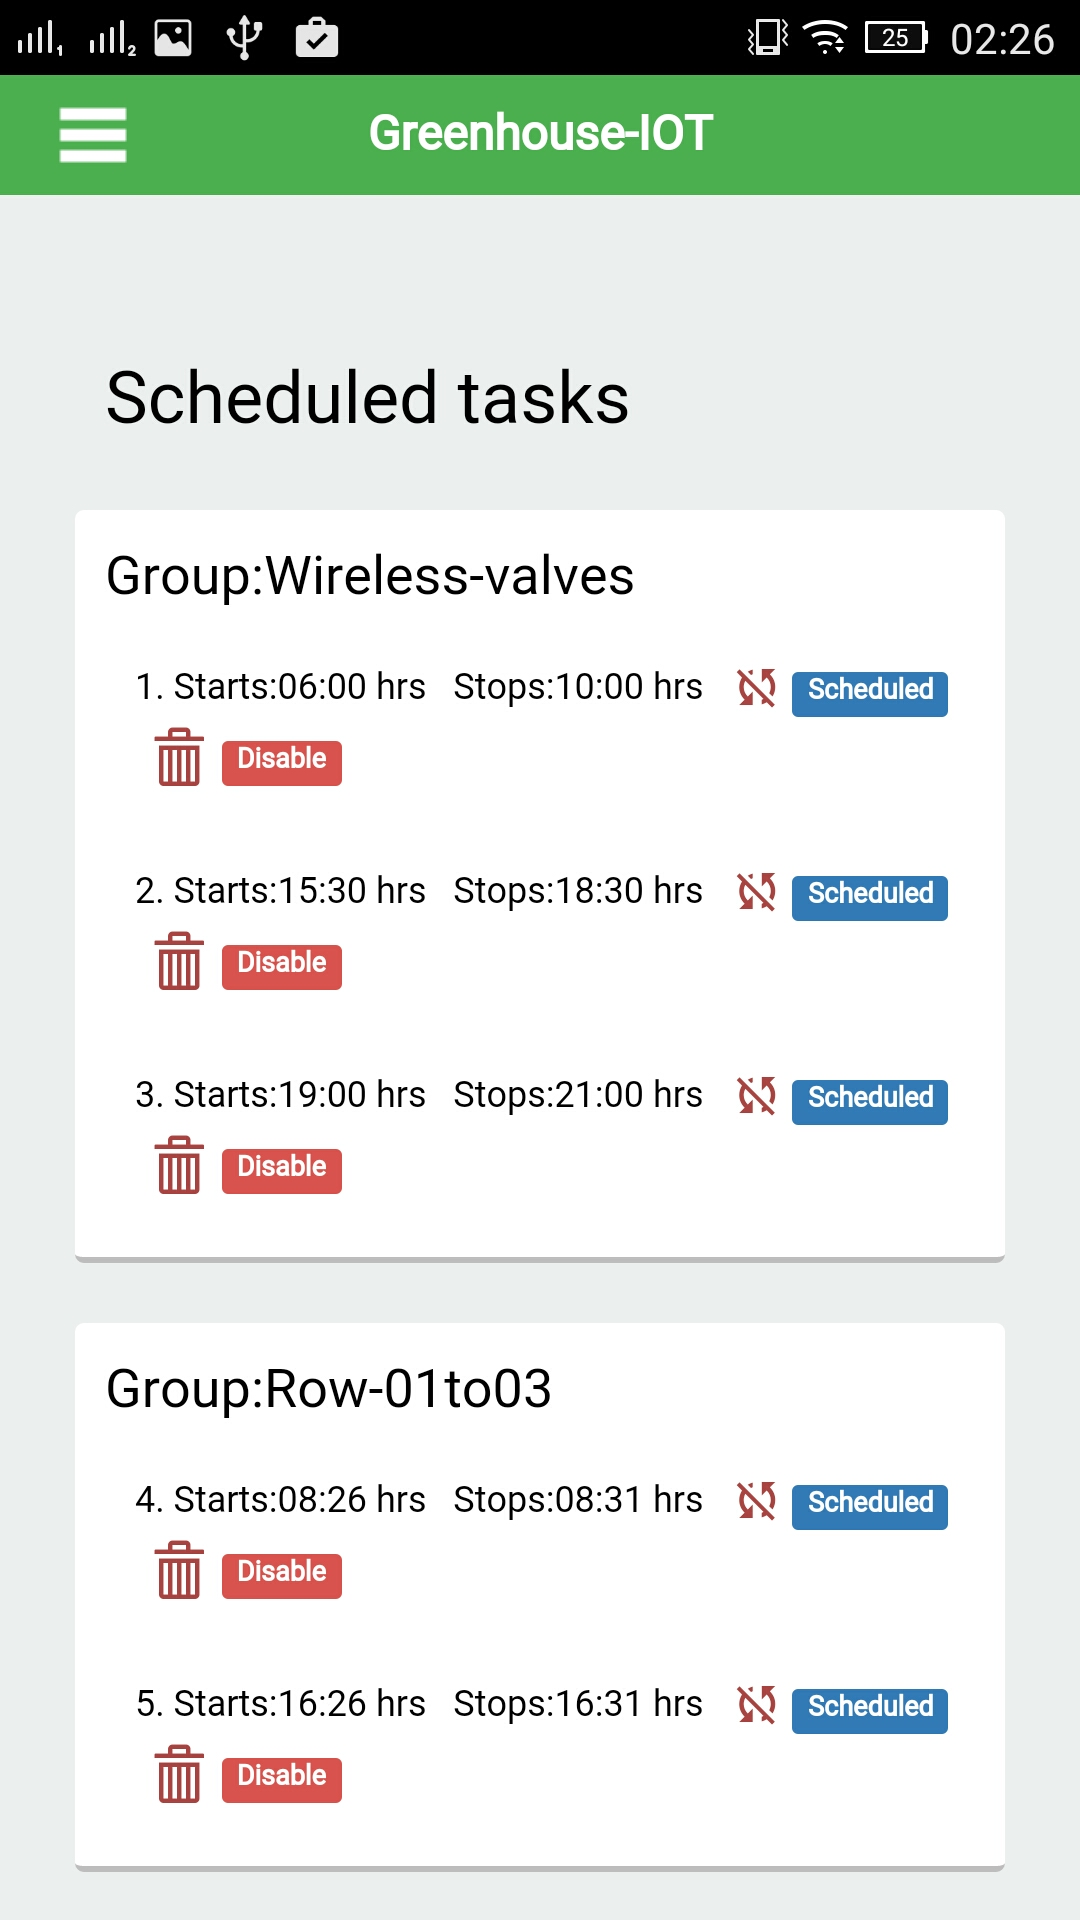
\includegraphics[width=10cm]{schedulingm.jpeg}
\newpage
Device Status Page\\

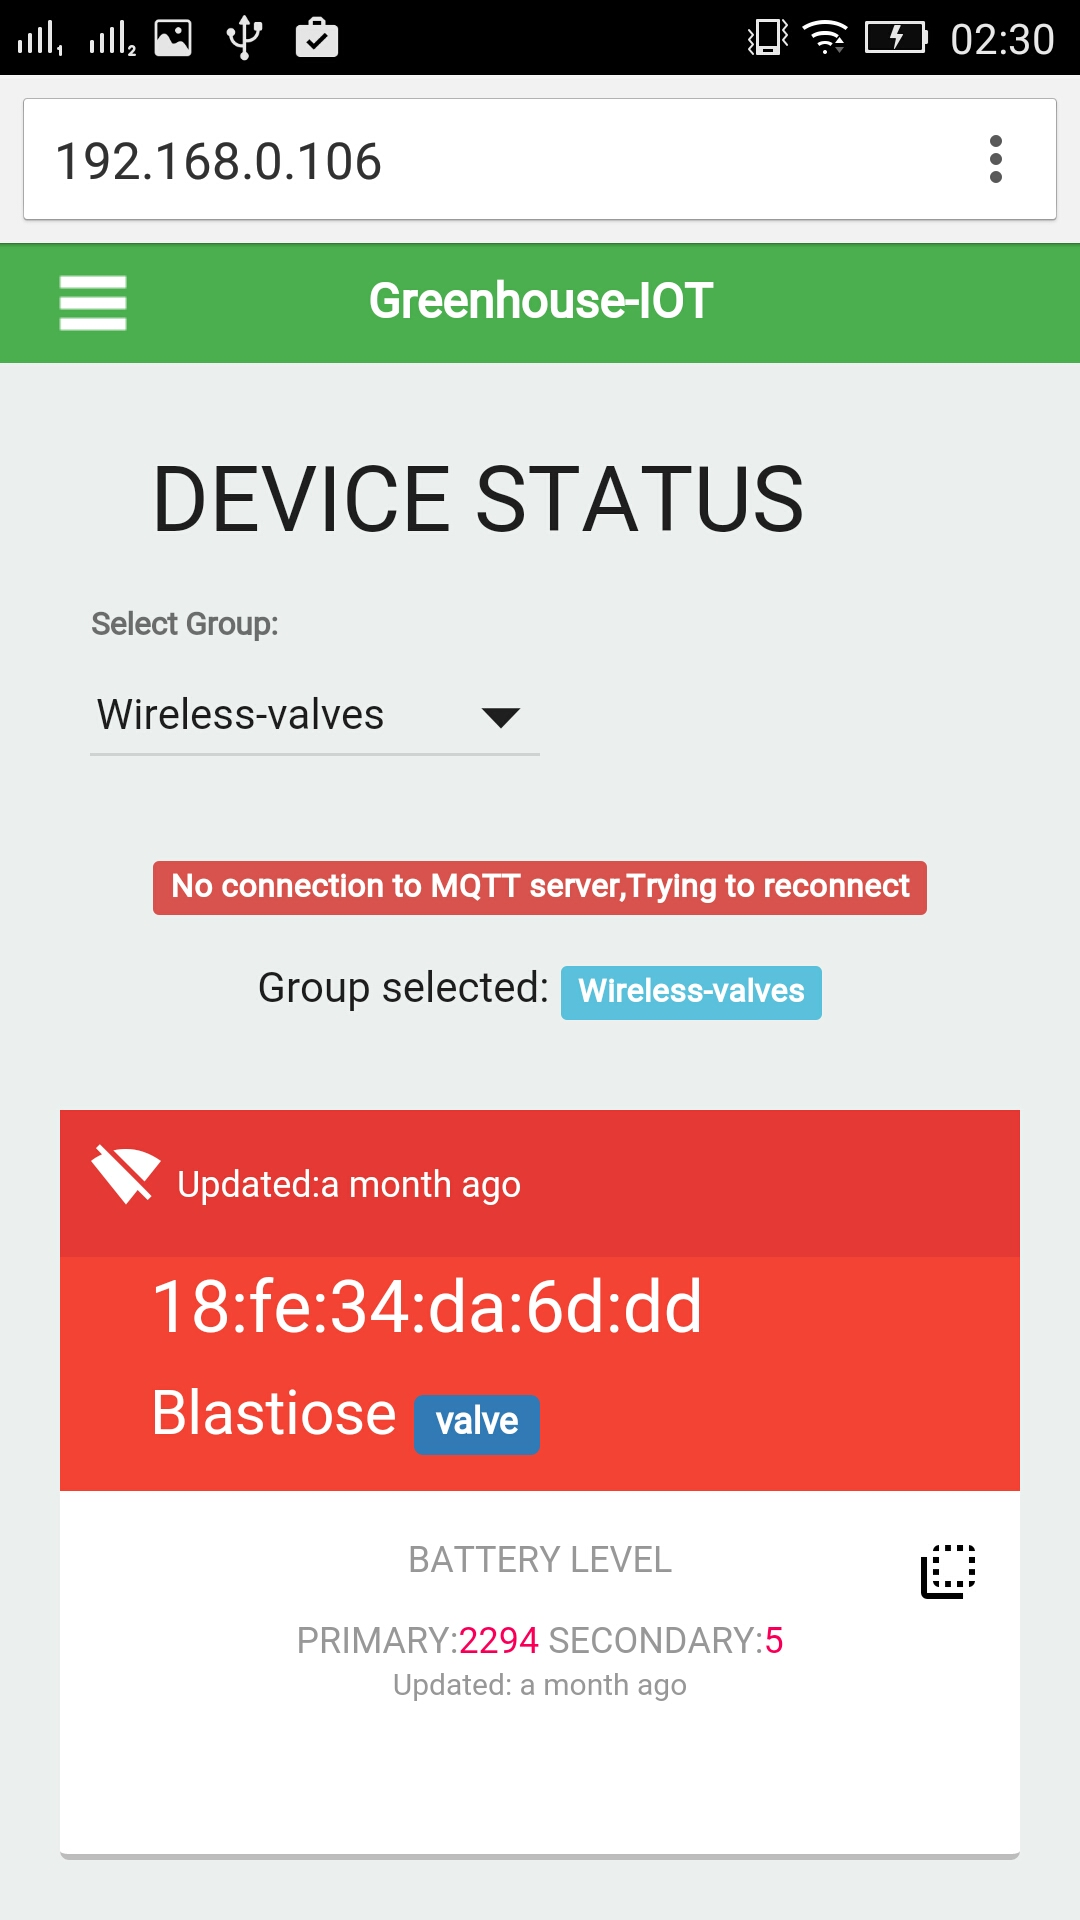
\includegraphics[width=10cm]{devicestatusm.jpeg}
\newpage
Valve Control Page\\

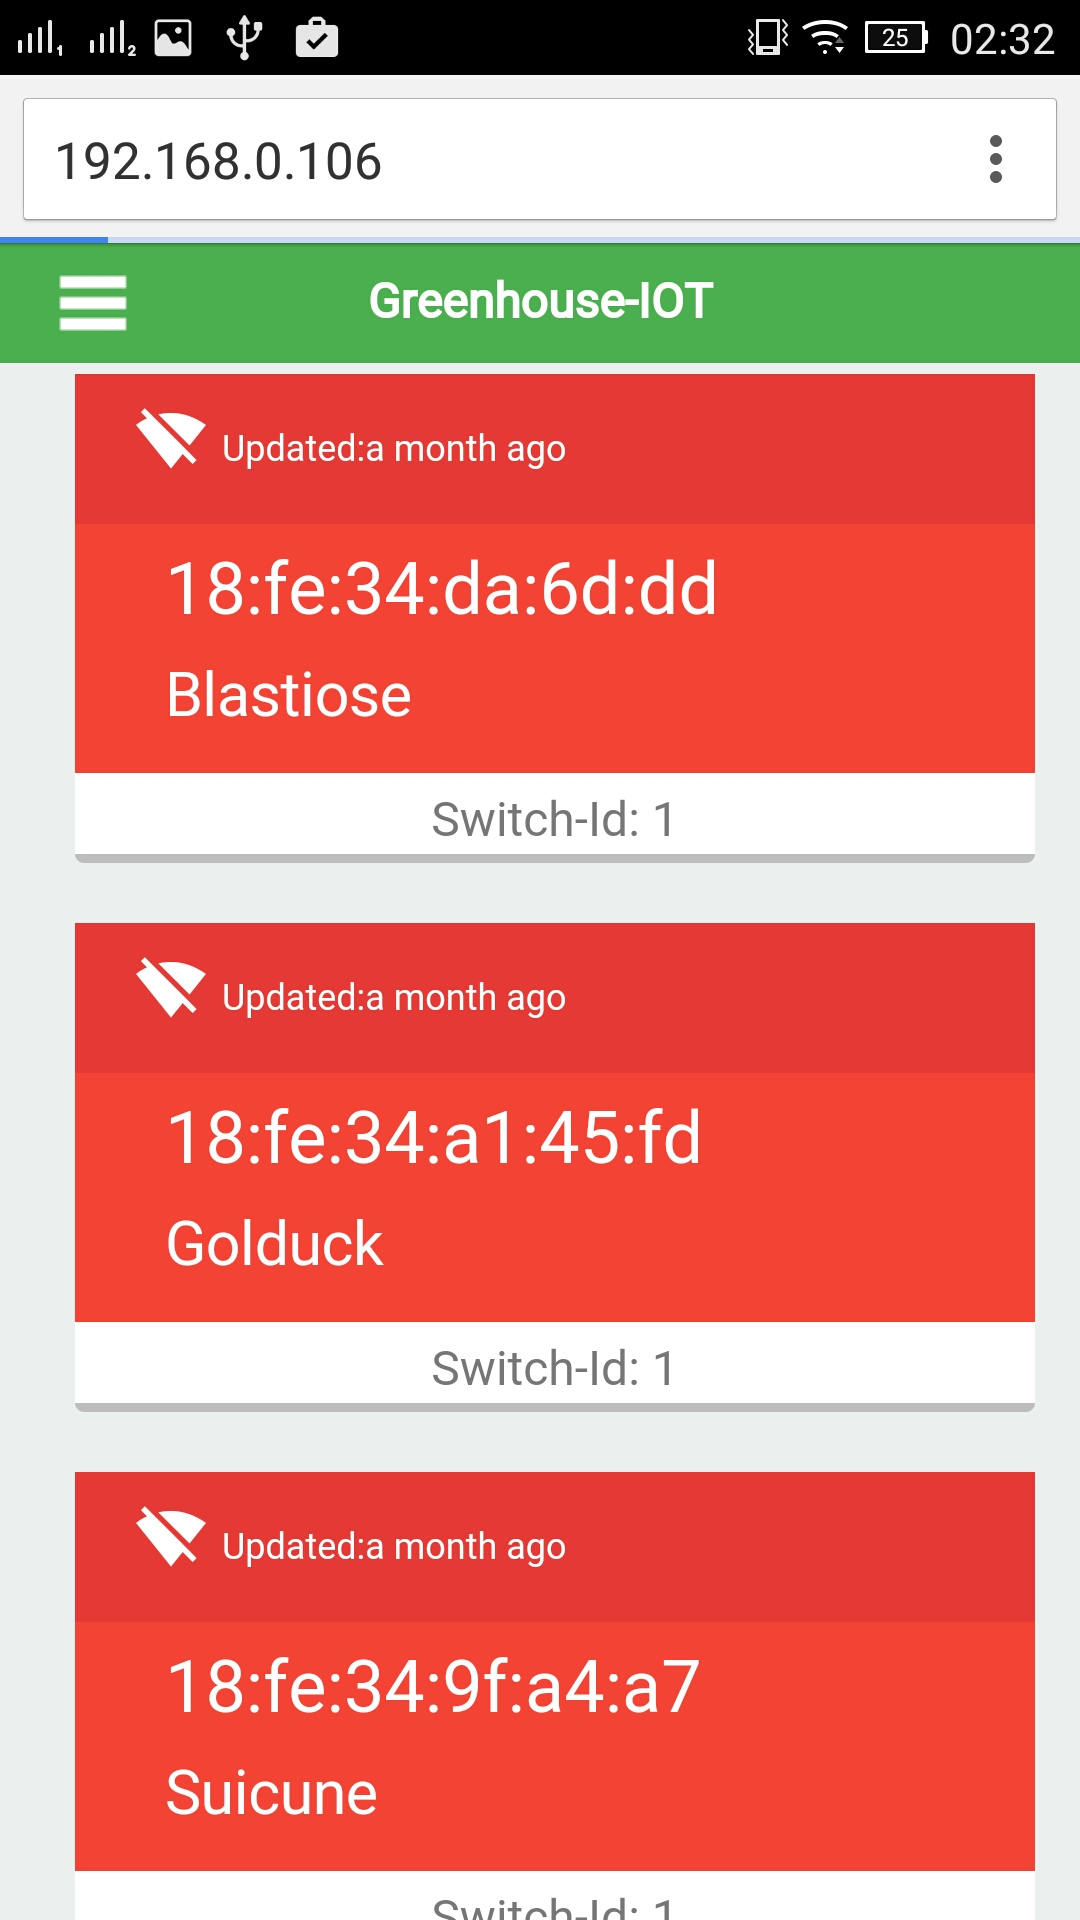
\includegraphics[width=10cm]{valvecontrolm.jpeg}
\newpage
Manage Users Page\\

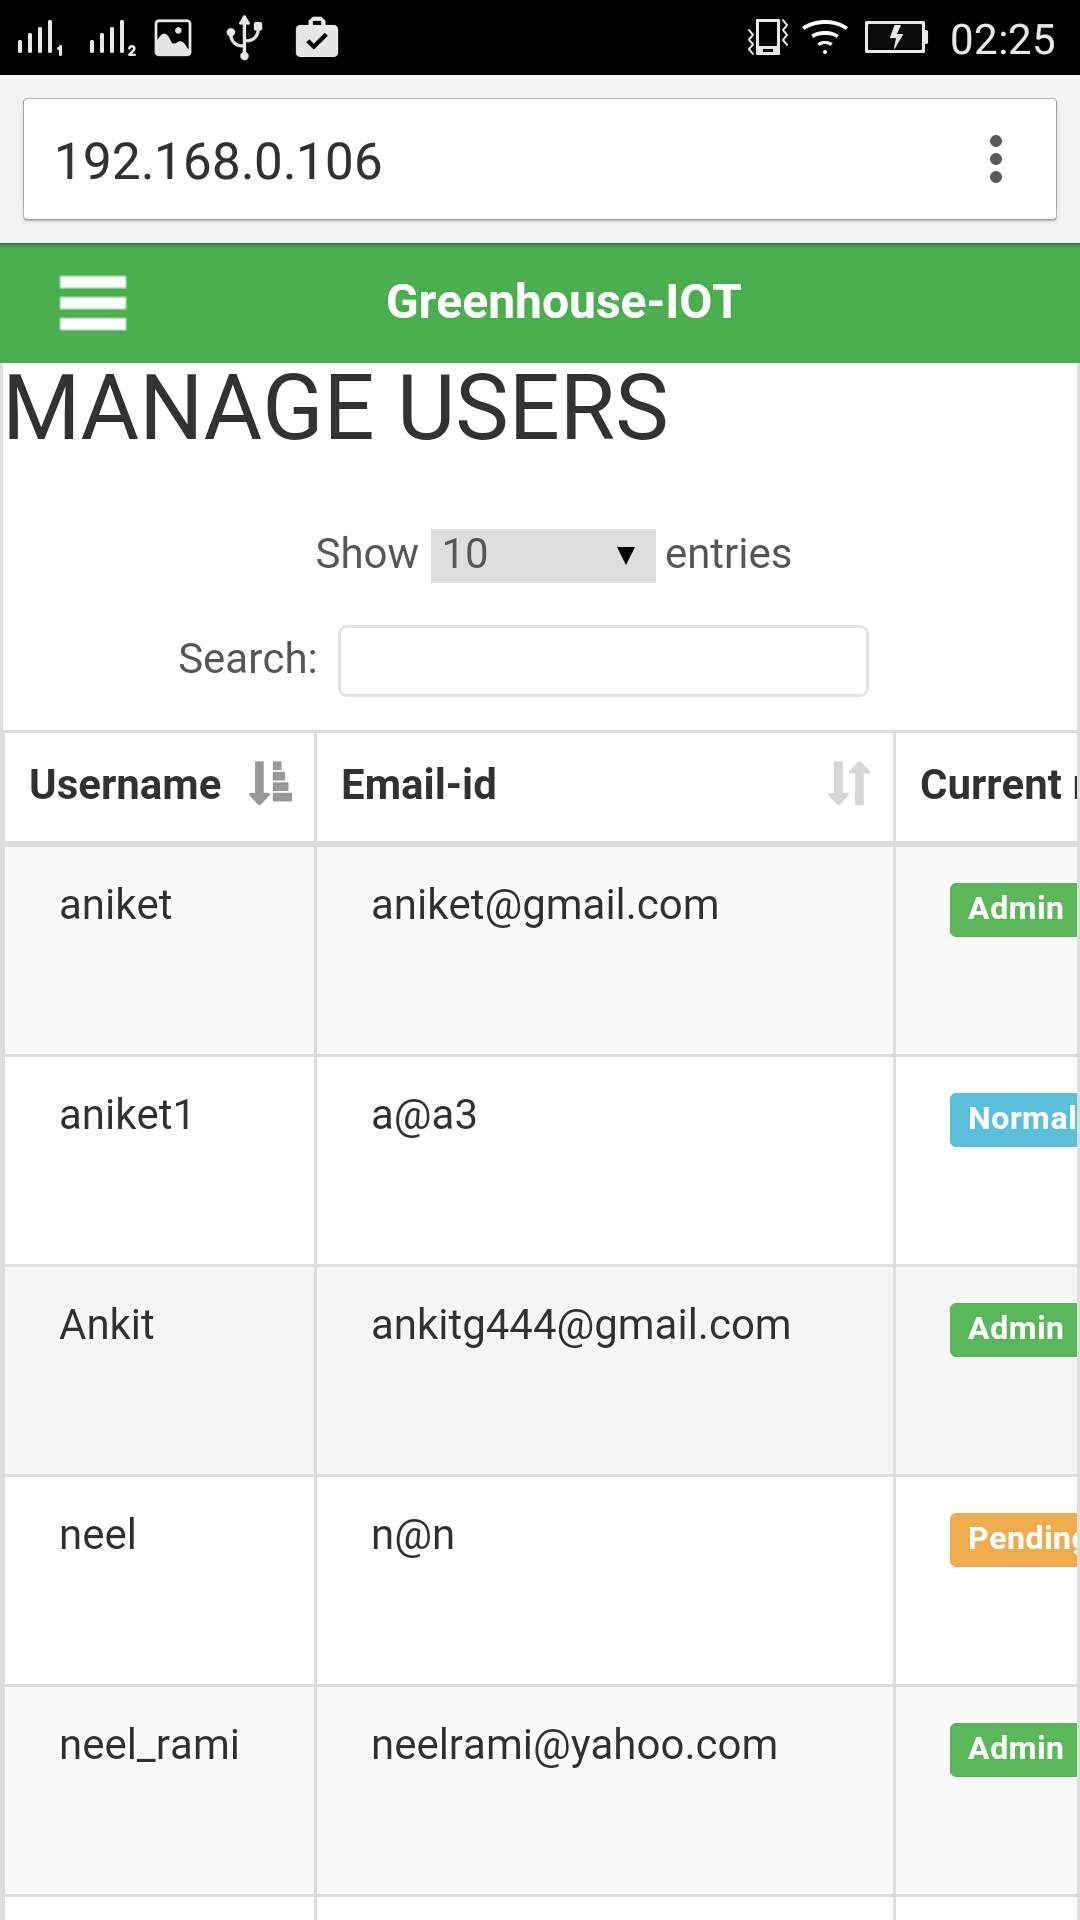
\includegraphics[width=10cm]{manageusersm.jpeg}
\newpage


\end{itemize}
 


\href{https://youtu.be/fZxgUEiySDY}{Youtube Link} of demonstration video 

\section{Future Work}
\begin{itemize}
\item{Large Scale Purpose}
\begin{itemize}
\item{Integrating the web portal with Greenhouse system and irrigation system.}
\end{itemize}
\item{Small Scale purpose}
\begin{itemize}
\item{{Automated watering of plants in gardens and houses.}}
\end{itemize}
\end{itemize}


\section{Bug report and Challenges}
\begin{itemize}
\item{Bugs}
\begin{enumerate}
    \item{Small UI flaws may be present.}
    \item{The site is vulnerable to web attacks such as SQL Injection etc.}
\end{enumerate}
\item{Challenges Faced}
\begin{enumerate}
    \item{Designing good UI.}
    \item{Implementing Websockets.}
    \item{Working with charts.}
\end{enumerate}
\item{Failures}
\begin{enumerate}
    \item{Embedding RTSP live video feed in a webpage.}
\end{enumerate}
    
    
\end{itemize}
\end{enumerate}


\begin{thebibliography}
\begin{itemize}
    \item{Stack Overflow}
    \item{TutorialsPoint}
    \item{TreeHouse}
    \item{Coursera}
    \item{Udemy}
    \item{GitHub}
    \item{Head First PHP \& MYSQL}
\end{itemize}

\end{thebibliography}


\end{document}

